\chapter{Conclusions and future developments}
In this concluding chapter, I present some final thoughts and propose potential directions for future research concerning the development of PEO ontology.


\section{Conclusions}
The work described in this thesis aimed to create a resource representing two recently emerged technologies: large language models and prompt engineering. Given the novelty of these technologies, existing resources are fragmented and outdated, lacking the latest developments. This highlighted the need to create a comprehensive resource that thoroughly represents prompt engineering and large language models, along with related aspects such as architecture, solvable tasks, functionalities of large language models, and prompts that can be crafted using prompt engineering techniques. Starting the project with two research questions in mind: "Is it possible to formalize the knowledge related to large language models and prompting techniques?" and "Is it possible to use the model formalization to get additional knowledge?" I delved into state-of-the-art techniques in ontology engineering and ontology design patterns to understand the process to follow during development and the concepts that could be reused in the representation.After completing this study, I proceeded to examine the main state-of-the-art large language models, including both general-purpose and multimodal models. Finally, I delved into prompt engineering, studying and describing the leading state-of-the-art techniques in this field. This comprehensive study, which explored multiple aspects, provided me with a clear framework of what should be represented in the ontology and the steps to follow for its development. Following the LOT (Linked Open Terms) methodology, widely used in the industry for ontology and vocabulary development, I defined the project requirements. This included considering possible use cases, identifying sources for the information to be included in the ontology, outlining functional and non-functional requirements, and determining the ontology's purpose and scope. All this information is compiled in a document called the ORSD (Ontology Requirements Specification Document), which is valuable for ontology developers or anyone seeking to understand the ideas and problems addressed by the ontology. The work continued with the conceptualization of the ontology, taking into account ontology design patterns. This was followed by encoding the ontology in RDF and TTL formats, creating all necessary classes and relationships, and adequately populating it with instances of the various classes. Since manually populating the ontology is a lengthy and tedious task, I experimented with using GPT-4 to automatically populate the ontology, resulting in a second version of the PEO ontology. Both versions of the PEO ontology are tested and their quality and consistency were verified against the requirements defined at the outset. The evaluation provided a comprehensive overview of the quality of the results achieved. The ontology is consistent, includes a substantial number of classes, is not overly complex, and is capable of correctly addressing the competency questions, which were translated into SPARQL queries. During the evaluation, some minor issues also emerged, specifically the presence of non-critical pitfalls detected by the OOPS! system, which were promptly addressed to ensure and improve the quality and accuracy of the ontology. Particular importance was also given to its publication; in fact, the ontology is indexed on W3id.org at the URL: \href{https://w3id.org/peo}{w3id.org/peo} making it easily accessible for everyone. All the source code of PEO ontology is available on \href{https://github.com/simonegramegna/peo}{Github repository} and the PEO ontology is also available on \href{https://bioportal.bioontology.org/ontologies/PEO_ONTOLOGY}{BioPortal}.\\
The PEO ontology stands as an innovative resource, never before developed within the vast landscape of ontologies and the semantic web. Although there have been modest attempts by other developers to create ontologies in this field, these efforts appear rather limited and incomplete compared to the PEO ontology, rendering them useless for any user. The careful, structured, and methodical development process, with the user and their needs in mind, has resulted in a high-quality ontology that is accessible to both expert and non-expert users. In the use cases formalized during the requirements definition, both expert and inexperienced users were taken into consideration. This ensures that the PEO ontology is not only a resource for those with solid knowledge and a strong foundation in the field of artificial intelligence and large language models but also for students or users with no prior knowledge who want to approach this field but don’t know where to start. The vast amount and variety of online resources can be daunting, particularly for beginners, who may feel overwhelmed by a "tsunami" of rapidly unfolding information driven by the fast pace of technological advancements. In this context, the PEO ontology serves as a reliable and comprehensive resource, capable of guiding both expert and inexperienced users through the landscape of large language models and prompt engineering, which are essential today for automating many repetitive tasks. The formalization, as described in the ontology implementation chapter, is complete and it considers only important aspects of the two filed without considering too technical aspects that cannot be understood by any user. The formalization in the ontology also enables the acquisition of new knowledge through inference, the inference is clear to the user and is carried out using property chains that combine multiple object properties into a single, inferred property.

\section{Future developments}
The future developments of the PEO ontology are numerous and can proceed in different but complementary directions to further enrich the PEO ontology. Among these, I consider as interesting future developments:
\begin{itemize}
    \item \textbf{Automatic population using LLMs:} this aspect was superficially explored during the experimentation phase. A potential area for development could involve experimenting with other LLMs and applying more advanced techniques for ontology population.

    \item \textbf{Integration with external ontologies:} the PEO ontology does not currently utilize or integrate any external ontologies related to large language models. Therefore, a potential research direction could involve exploring how to integrate the information from these ontologies into the PEO ontology.

    \item \textbf{Improvement of the inference part:} the PEO ontology includes property chains for inference. A potential future development could involve improving and extending this aspect to infer new information based on the knowledge already encoded in the PEO ontology.

    \item \textbf{Database integration:} an interesting future development could be the integration of the PEO ontology with relational and non-relational databases to enrich the databases with the semantics provided by the ontology and facilitate interoperability with other information sources.

    \item \textbf{PEO ontology web application:} the development of a web application using HTML, CSS, and JavaScript to interact with the PEO ontology is a potential future advancement that could enhance its accessibility and support its wider adoption. 
\end{itemize}
The future developments that will be carried out will surely enhance the PEO ontology project, a unique project never experimented that was casually born during a Teams call with my advisor on a warm day in mid-May 2024.

\begin{figure}[H]
    \centering
    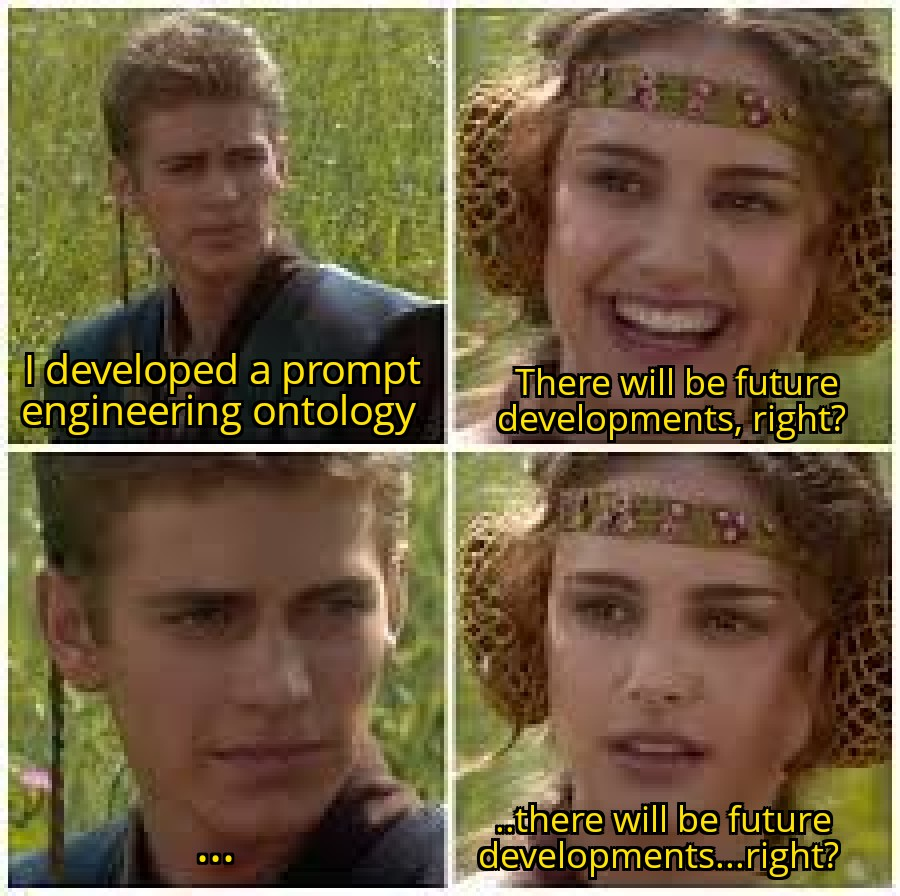
\includegraphics[width=0.5\linewidth]{Figures/fig_84.jpg}
\end{figure}